\section{Pascal Analyzer validation} \label{sec:pascal_framework_validation}
In this Section, we discuss the measurements and simulation results for three distinct cases, including two real applications. We also demonstrate how external libraries and standalone visualization tools can be used to render the collected data and investigate performance aspects such as the program's scalability capacity.

We used three experiments to assess the tool and demonstrate its ability to support analysis aimed at observing parallel scalability. The first includes a runtime imbalance between processing units in a specific parallel region. In this case, the objective is to present how the analyzer helps users observe the impact of the inefficiency of a code part on the whole program. The code for this experiment is presented in \cref{lst:codes_regionscomparison}. It consists of two simple parallel regions with the same functionality that divide the iterations of a loop between the available threads. The difference between the regions lies in the strategies used to manipulate the sum variable, used in the example to store the values of the calculations performed in each thread. We assume that the {\tt anyop()} function, in this case, invariably has the same runtime in all function calls.

The command presented on \cref{lst:pascal_usage_ex} was used as base to perform experiments. For the experiment of \cref{lst:codes_regionscomparison}, we use just the parameters {\tt -c}, {\tt -r}, {\tt -t}, {\tt -a} and {\tt -o}, including the 64 value to {\tt -c} option.

\lstset{style=ccodestyle, frame=tb}
\begin{lstlisting}[label={lst:pascal_usage_ex}, language=bash, caption={Command line showing how experiments were run through a terminal.}]
	analyzer 
	application
	-c 1,2,4,8,...,32 # threads/cores
	-r 3 # number of repetitions
	-t auto # automated instrumentation
	-a 1 # aggregation mode
	--ipmi ip user psswd # energy sensor
	--idtm 5 # idle time between runs
	--dhpt # disable hyper-thread
	--dcrs # disable cores
	--ipts ... # application specific inputs
	-o application.json # output file
\end{lstlisting}

\lstset{style=ccodestyle, frame=tb}
\begin{lstlisting}[label={lst:codes_regionscomparison}, language=C, caption={Sample code used to visualize the impact of regions on program scalability.}]
	int main(int argc, char **argv) {
		unsigned long sum = 0;
		int ops = atoi(argv[1]);
		
		#pragma omp parallel for schedule(static) reduction(+: sum)
		for (int i = 0; i < ops; i++)
		sum += anyop();
		
		#pragma omp parallel for schedule(static)
		for (int i = 0; i < ops; i++) {
			#pragma omp critical
			sum += anyop();
		}
	}
\end{lstlisting}

The command return a .json file with all the information necessary for our analysis. We can quickly generate tables with the collected data from this file, thus supporting observation and analysis of scalability, energy trends, and model fitting. The code described in \cref{lst:regtab} and \cref{tab:regtable_dedup} are samples of how users can easily read and view collected data from the control terminal in a tabular way.

\lstset{style=pythonStyle, frame=tb}
\begin{lstlisting}[label={lst:regtab}, language=python, captionpos=b, caption={Example of using the Python API to load analyzer files.}]
	from analyzer import Data
	
	data = Data("application.json")
	data.energy(regions=True)
	# data.speedup()
	# data.efficiency()
	# data.regions()
\end{lstlisting}

%The result can be seen in tabular form, as shown in Table.~\ref{tab:regtable_dedup}. Using these tables, we can quickly generate figures showing the application's behavior from various points of view. In Figures \ref{fig:speedup_raytrace} and \ref{fig:speedup_openmc} we observe the trend of the speedup with the number of cores and input.
\begin{table}[H]
	\caption{Dataframe generated automatically from collected samples using the Python API.}
	\label{tab:regtable_dedup}
	
	\resizebox{\columnwidth}{!}{%
		\begin{tabular}{ccccccc}
			\toprule
			\textbf{Repetition} & \textbf{Input} & \textbf{Cores} & \textbf{Regions} & \textbf{Start Time (s)} & \textbf{Stop Time (s)} & \multicolumn{1}{c}{\textbf{ipmi Energy (J)}} \\ \midrule
			1 & 1 & 1 & 1 & 0.00 & 66.31 & 13,156.19 \\
			1 & 1 & 1 & 2 & 0.00 & 66.27 & 13,148.87 \\
			... & ... & ... & ... & ... & ... & ... \\
			1 & 5 & 30 & 4 & 0.00 & 8.46 & 1903.82 \\
			1 & 5 & 30 & 5 & 0.02 & 58.16 & 13,067.01 \\ \bottomrule
	\end{tabular}}
\end{table}

\subsection{Case of study}\label{subsec:pfv_case_of_study}

The analyzer does not display graphics and other visual elements natively. However, the simple use of external libraries allows generating graphics and visualizing points of the program's behavior that you want to observe. In addition, specialized visualization tools can also be used to view the results. PaScal Viewer \cite{Silva2018}, for example, natively interprets the analyzer's output files, complementing its functionality and creating an integrated and appropriate environment for the program's parallel scalability analysis.

To analyze the experiment presented in \cref{lst:codes_regionscomparison}, we use PaScal Viewer to observe in a hierarchical way how the different OpenMP clauses impacted the region's efficiencies. The efficiency pinpoints how a program can take advantage of increasing processing elements on a parallel system. It is defined as the ratio of speedup to the number of processing units. In this sense, PaScal Viewer displays an efficiency diagram for each analysis region, as presented in \cref{fig:pv_regionscomparison}. Comparing these diagrams, it is possible to see how the critical clause damages the scalability. In addition, it is also possible to relate that this second region affects the efficiency of the whole program due to the code characteristics.

If the reduction clause replaces {\tt \#pragma~omp~crtical}, the second region and the entire program become more efficient, as shown in \cref{fig:pv_regionscomparison_2}. The PaScal Viewer diagrams mentioned in this work, the x-axis (i1--i7) corresponds to different data inputs and the y-axis (2--64) to the number of threads used in the processing. Figures~\ref{fig:pv_regionscomparison} and \ref{fig:pv_regionscomparison_2} were rendered using a tool feature that smoothes the color transition of diagrams. This feature uses interpolation to create a visual element where the color transition is less pronounced. The diagram axes only show the initial and final values with this option. The user can visualize diagrams with only discrete values or even compare the two presentation modes side by side. \cref{fig:visualizationmodes} shows the difference between discrete and smoothed modes considering the whole program and the simulation scenario that uses the clause {\tt \#pragma~omp~crtical}.
\begin{figure}[H]
	\begin{subfigure}[b]{0.45\textwidth}
		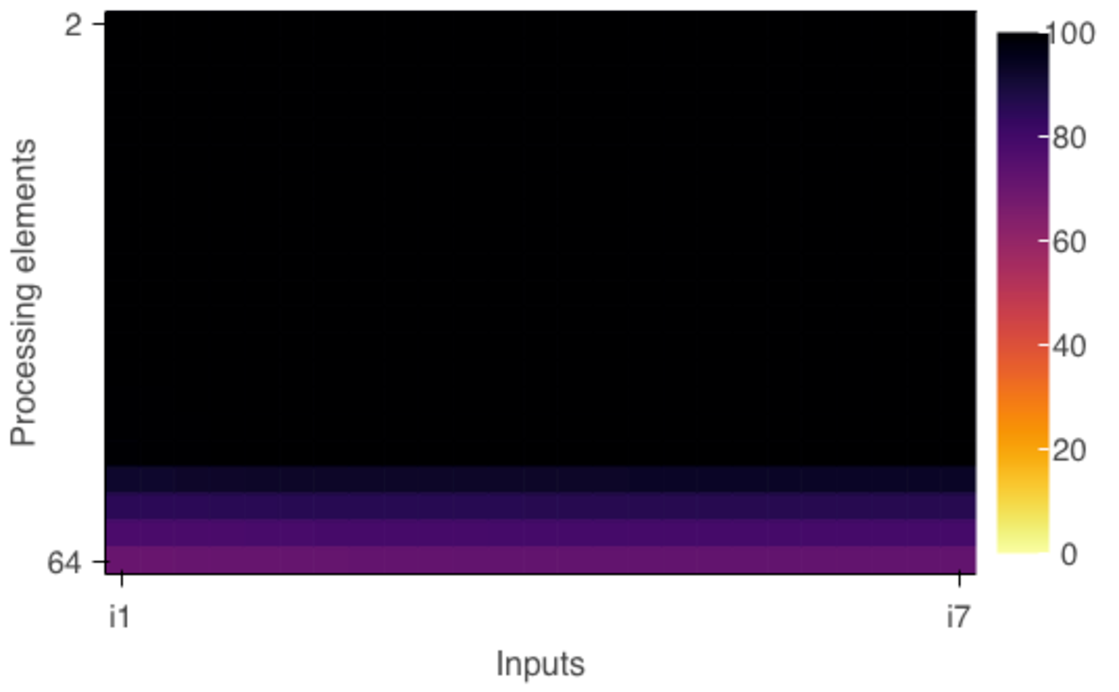
\includegraphics[width=\textwidth]{pascalanalyzer/figures/results/regionscomparison_r1.pdf}
%		\caption{\centering}
		\label{fig:pv_regionscomparison_a}
	\end{subfigure}
	\begin{subfigure}[b]{0.45\textwidth}
		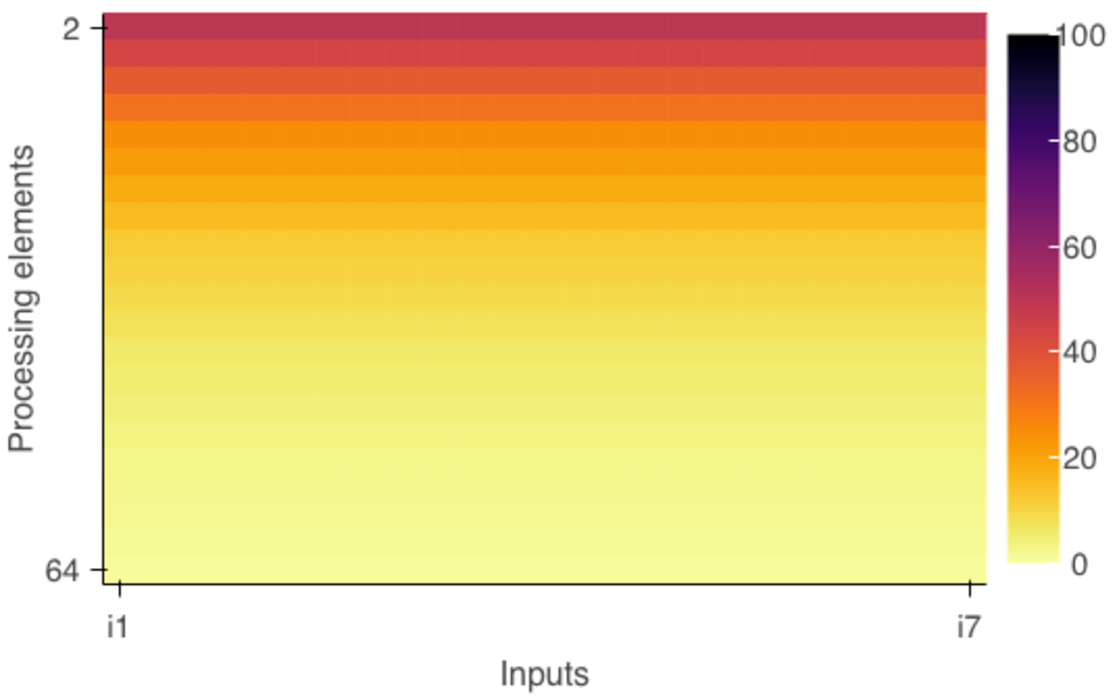
\includegraphics[width=\textwidth]{pascalanalyzer/figures/results/regionscomparison_r2.pdf}
%		\caption{\centering}
		\label{fig:pv_regionscomparison_b}
	\end{subfigure}
	\begin{subfigure}[b]{0.45\textwidth}
		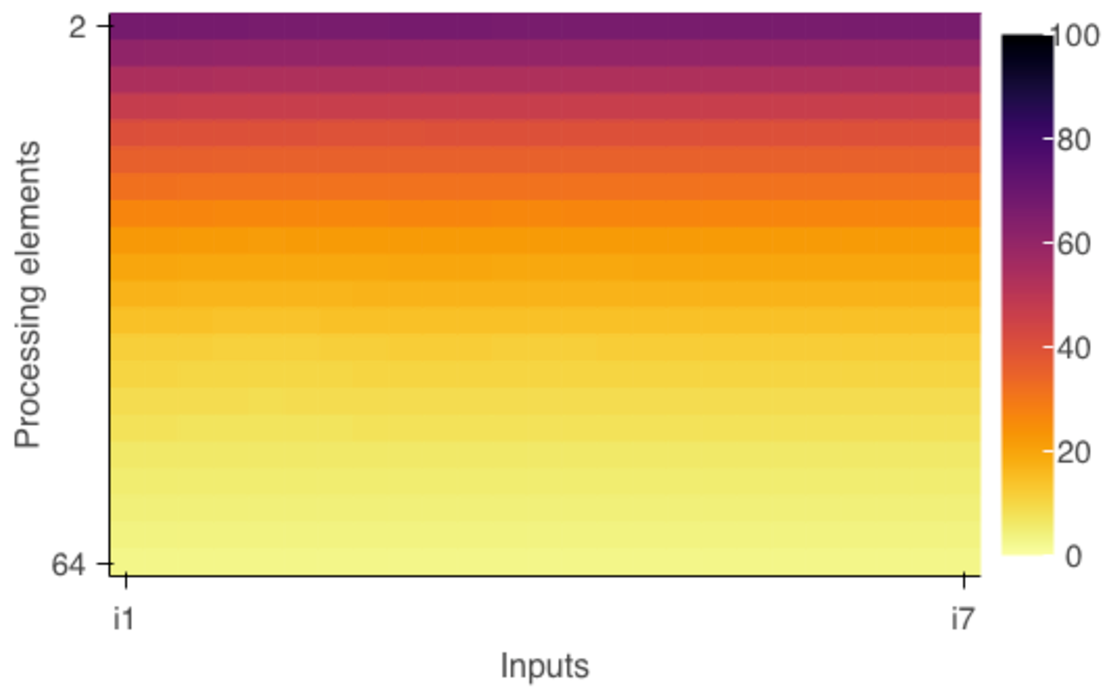
\includegraphics[width=\textwidth]{pascalanalyzer/figures/results/regionscomparison_whole.pdf}
%		\caption{\centering}
		\label{fig:pv_regionscomparison_c}
	\end{subfigure}
	\caption{Efficiency diagrams and impact of inner regions on program scalability. (x-axis = inputs; y-axis = number of threads). (\textbf{a}) First region diagram. (\textbf{b}) Second region diagram. (\textbf{c}) Whole program~diagram.}
	\label{fig:pv_regionscomparison}
\end{figure}
\unskip
\begin{figure}[H]
	\begin{subfigure}[b]{0.45\textwidth}
		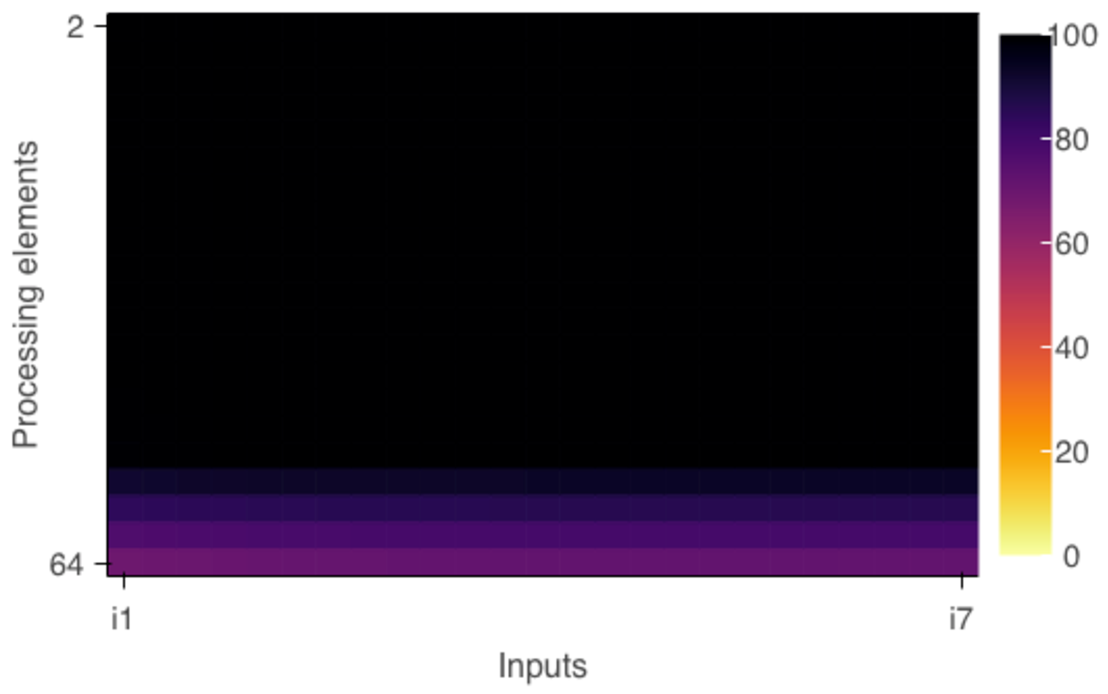
\includegraphics[width=\textwidth]{pascalanalyzer/figures/results/efficiency_rg_1.pdf}
%		\caption{\centering}
		\label{fig:pv_regionscomparison_a_2}
	\end{subfigure}
	\begin{subfigure}[b]{0.45\textwidth}
		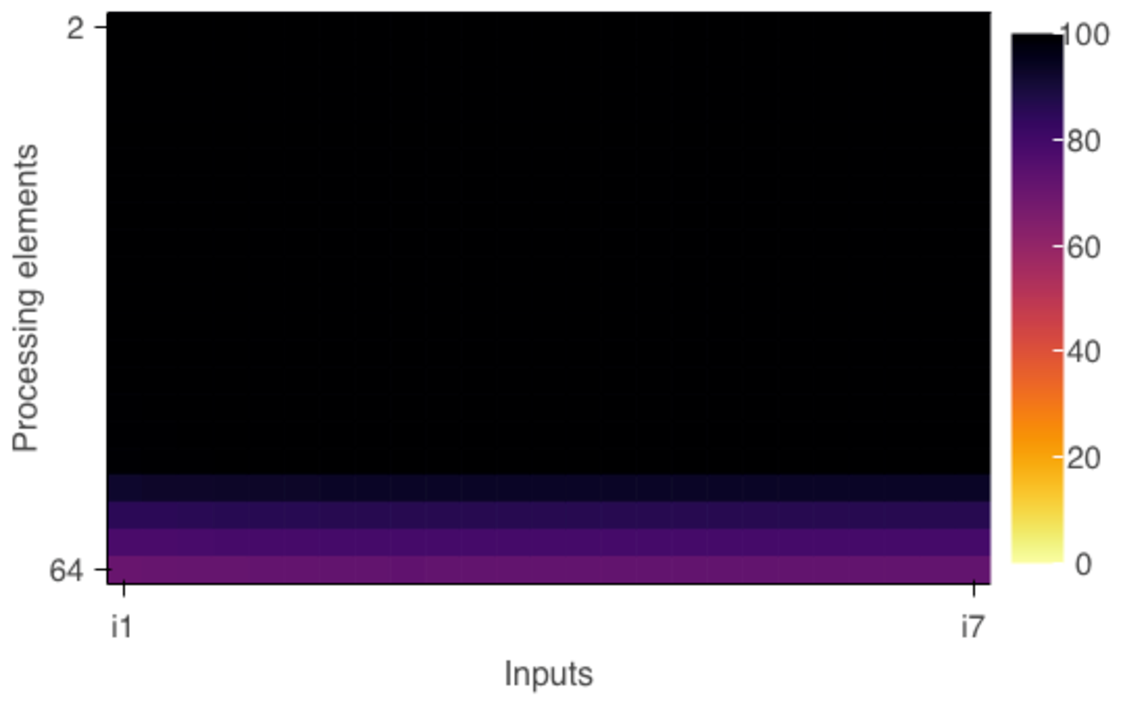
\includegraphics[width=\textwidth]{pascalanalyzer/figures/results/efficiency_rg_2.pdf}
%		\caption{\centering}
		\label{fig:pv_regionscomparison_b_2}
	\end{subfigure}
	\begin{subfigure}[b]{0.45\textwidth}
		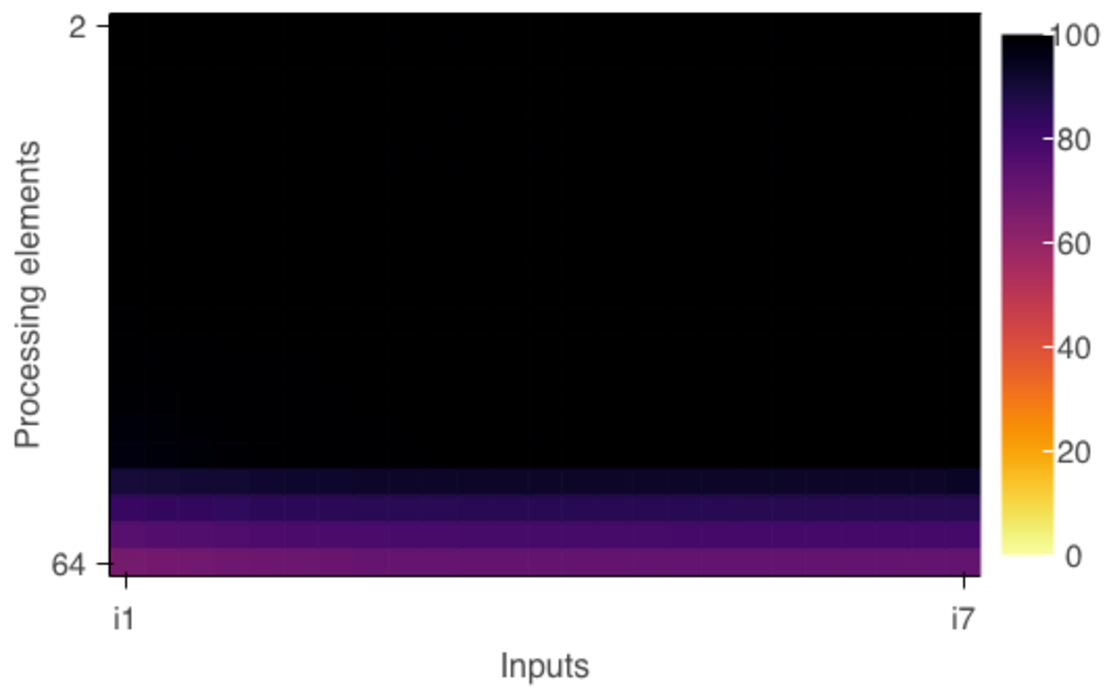
\includegraphics[width=\textwidth]{pascalanalyzer/figures/results/efficiency_rg_3.pdf}
%		\caption{\centering}
		\label{fig:pv_regionscomparison_c_2}
	\end{subfigure}
	\caption{Efficiency diagrams after removing {\tt \#pragma~omp~crtical} clause. (x-axis = inputs; y-axis = number of threads). (\textbf{a}) First region diagram. (\textbf{b}) Second region diagram. (\textbf{c}) Whole program~diagram.}
	\label{fig:pv_regionscomparison_2}
\end{figure}
\unskip
\begin{figure}[H]
	\begin{subfigure}[b]{0.45\textwidth}
		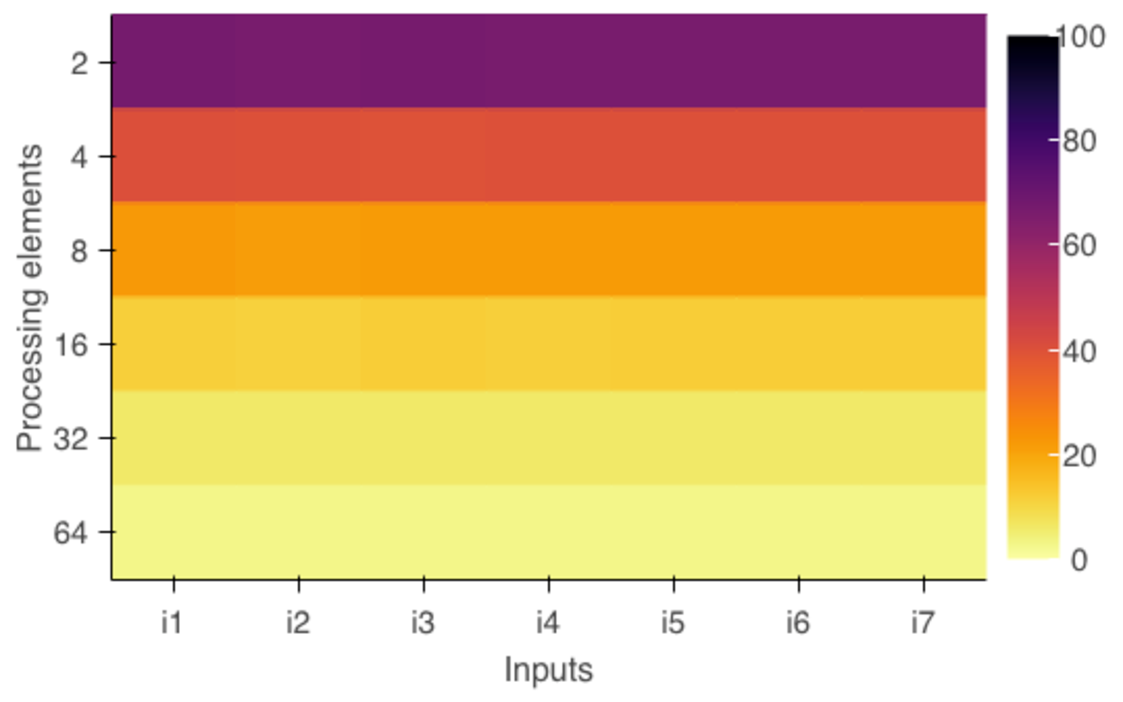
\includegraphics[width=\textwidth]{pascalanalyzer/figures/results/diagram_discretevalues.pdf}
%		\caption{\centering}
		\label{fig:discretevalues}
	\end{subfigure}
	%
	\begin{subfigure}[b]{0.45\textwidth}
		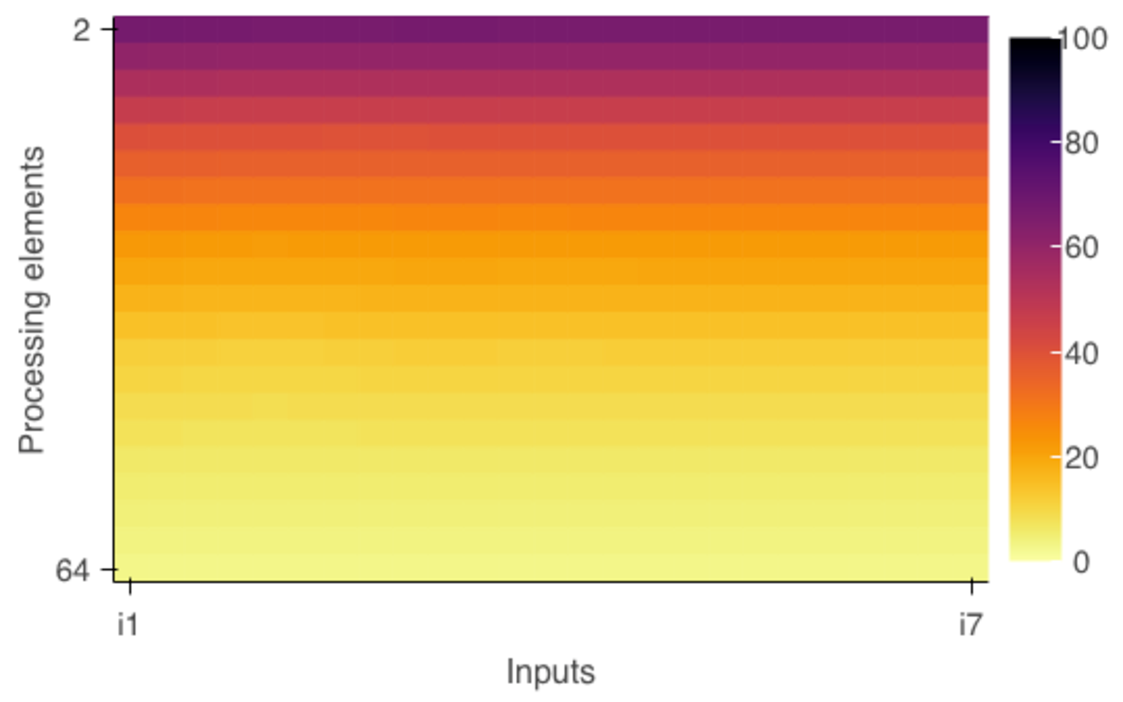
\includegraphics[width=\textwidth]{pascalanalyzer/figures/results/diagram_smoothedvalues.pdf}
%		\caption{\centering}
		\label{fig:smoothedvalues}
	\end{subfigure}
	
	\caption{Visualization modes of diagrams provided by PaScal Viewer. (\textbf{a}) PaScal Viewer diagram on discrete mode. (\textbf{b}) PaScal Viewer diagram on smoothed mode.}
	\label{fig:visualizationmodes}
\end{figure}


%The analyzer allows that the result can be seen in tabular form, as shown in Table.~\ref{tab:regtable_dedup}. Using these tables, we can quickly generate figures that show the application's behavior from various points of view. In Figures \ref{fig:speedup_raytrace} and \ref{fig:speedup_openmc} we can observe the trend of the speedup with the number of cores and input.

%Figures \ref{fig:raytrace_en} and \ref{fig:openmc_en} present the energy variation with the number of cores.

\textls[-19]{Other analysis objectives not supported by PaScal Viewer, such as visualization of the speedup curve or energy consumption, can be supported by traditional plots. Figures~\ref{fig:speedup} and \ref{fig:energy}} present the charts rendered for analysis by Raytrace and OpenMC applications. In these figures, it is possible to observe that the program efficiency varies according to the increase in the number of threads and the execution of inputs with higher processing loads. From the diagrams in \cref{fig:efficiency_all}, it is possible to observe that the applications present different behaviors concerning their efficiency variations and their scalability capabilities. OpenMC maintains its efficiency almost constant. This pattern represents strong scalability and indicates that the program can maintain its efficiency level when it uses a larger number of threads and processing larger inputs. On the other hand, \cref{fig:efficiency_all}a demonstrates that Raytrace achieves higher efficiency values when processing larger inputs. However, it is also possible to observe that increasing the number of processing units fixing the input size will not improve or hold the efficiency value.
\begin{figure}[H]
	\begin{subfigure}[b]{0.45\textwidth}
		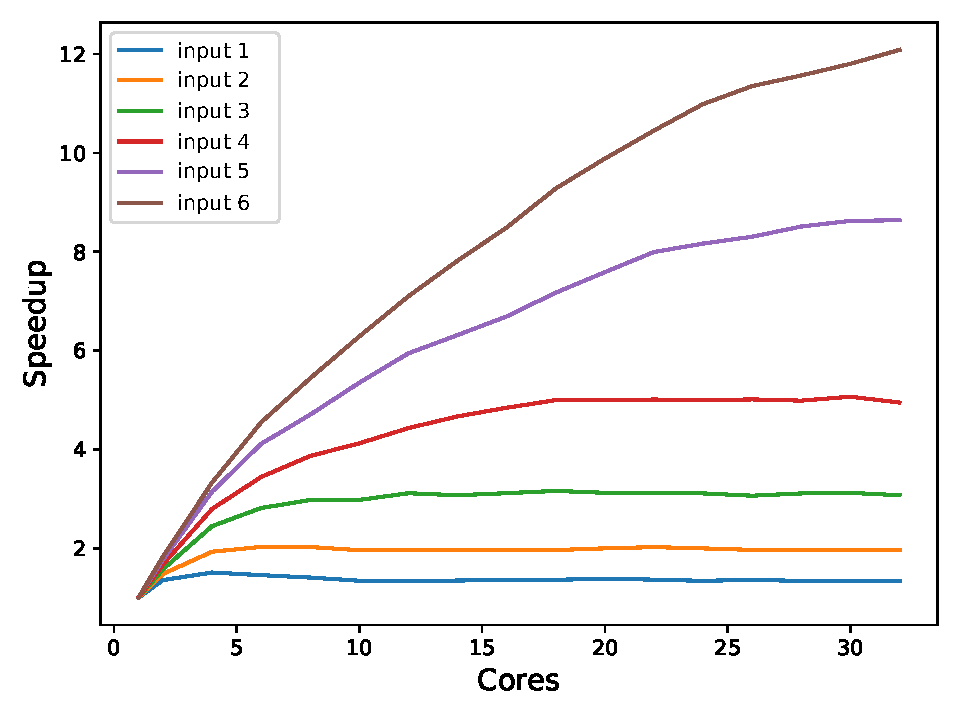
\includegraphics[width=\textwidth]{pascalanalyzer/figures/results/speedup_completo_rtview_2 (1).pdf}
%		\caption{\centering}
		\label{fig:speedup_raytrace}
	\end{subfigure}
	%
	\begin{subfigure}[b]{0.45\textwidth}
		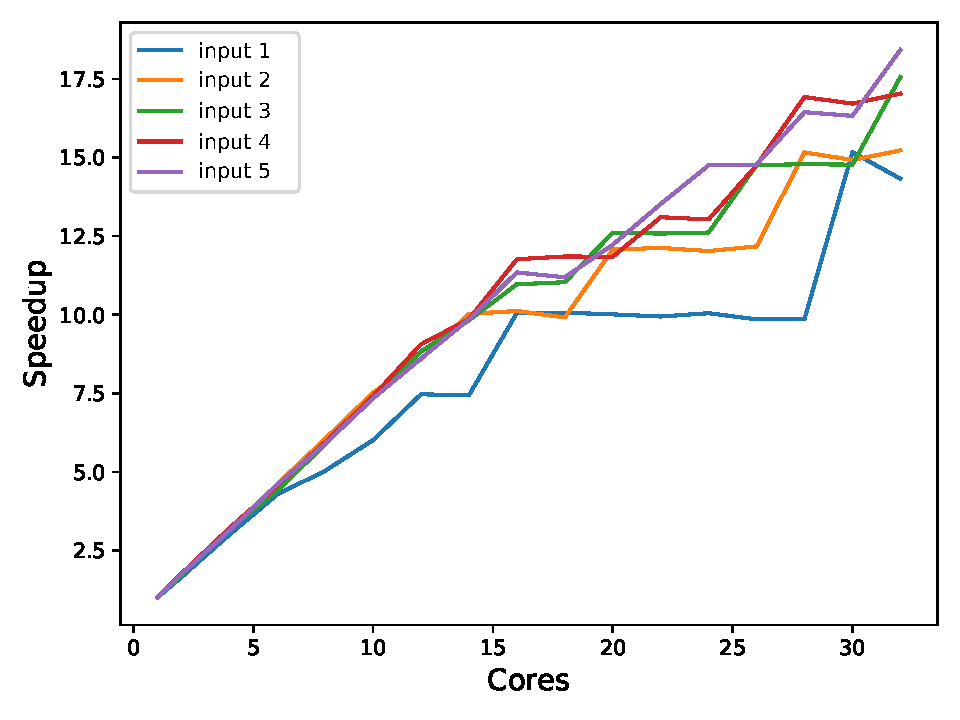
\includegraphics[width=\textwidth]{pascalanalyzer/figures/results/speedup_completo_openmc_kernel_novo (1).pdf}
%		\caption{\centering}
		\label{fig:speedup_openmc}
	\end{subfigure}
	\caption{\textls[-30]{Speedup of the applications for several input sizes. (\textbf{a}) Raytrace speedup. (\textbf{b}) OpenMC speedup. }}
	\label{fig:speedup}
\end{figure}
\unskip
\begin{figure}[H]
	\begin{subfigure}[b]{0.46\textwidth}
		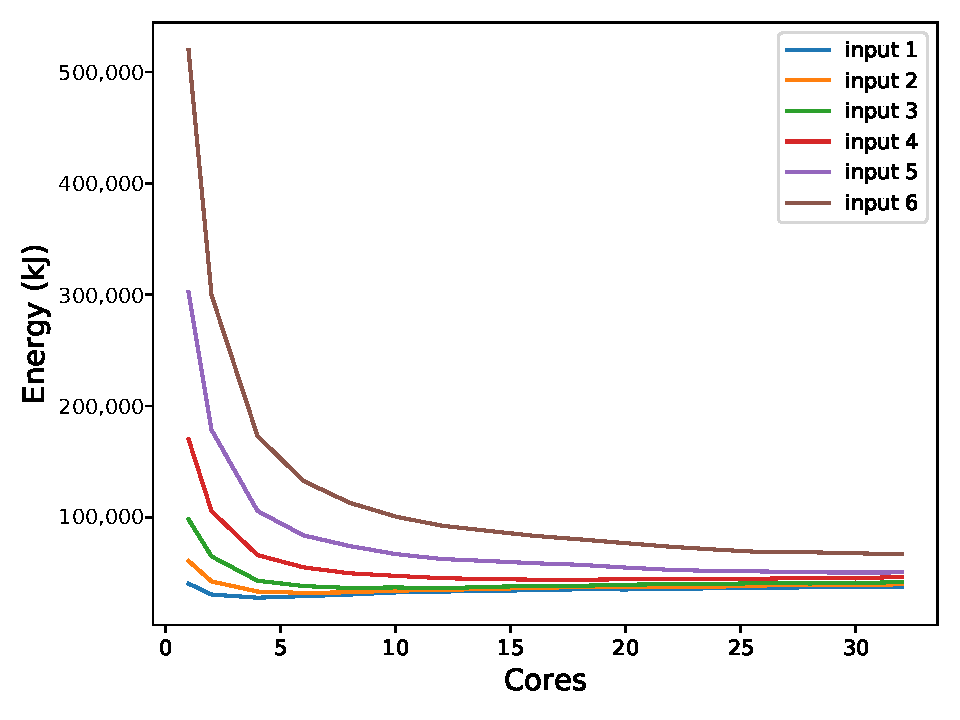
\includegraphics[width=\textwidth]{pascalanalyzer/figures/results/energy_completo_rtview_2 (1).pdf}
%		\caption{\centering}
		\label{fig:raytrace_en}
	\end{subfigure}
	%
	\begin{subfigure}[b]{0.46\textwidth}
		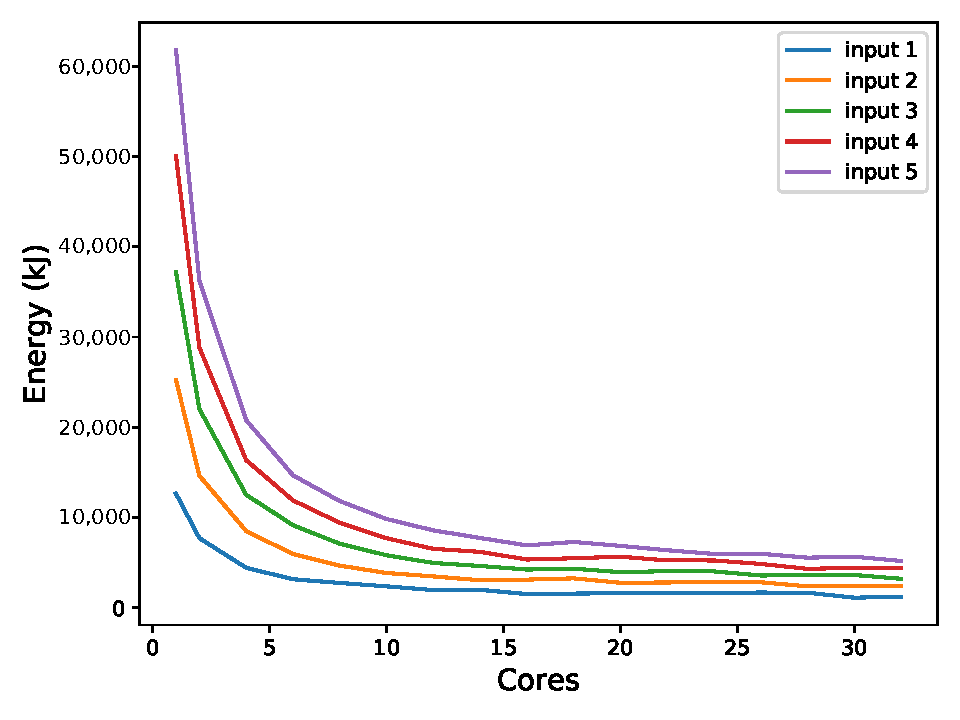
\includegraphics[width=\textwidth]{pascalanalyzer/figures/results/energy_completo_openmc_kernel_novo (1).pdf}
%		\caption{\centering}
		\label{fig:openmc_en}
	\end{subfigure}
	
	\caption{Energy consumption identified in the execution of applications while varying the number of cores for several input sizes.
		%MDPI: Please add commas to numbers to indicate thousand on the Oy axis of the figures, e.g. 20,000 30,000 40,000.
		(\textbf{a}) Raytrace energy consumption. (\textbf{b}) OpenMC energy consumption.}
	\label{fig:energy}
\end{figure}
\unskip
%Furthermore, using an external graphical interface module, we can load the .json file and intuitively visualize the program's scalability showing the efficiency. The efficiency pinpoint how efficiently a program can take advantage of increasing processing elements on a parallel system. It is defined as the ratio of speedup to the number of processors.
%For example, Figure \ref{fig:efficiency_all} shows examples of graphics generated for the same applications as above. In these figures, it is possible to observe that the program efficiency varies according to the increase in the number of threads and the execution of inputs with higher processing loads. From the Figure \ref{fig:efficiency_raytrace} we can see that as we increase the input size, the efficiency increases while slowly decreasing when the number of cores grows, indicating a tendency for a scalable program. In the second Figure \ref{fig:efficiency_openmc} the efficiency is practically constant while varying the number of cores and the input indicating a strong scalable program.
\begin{figure}[H]
	\begin{subfigure}[b]{0.46\textwidth}
		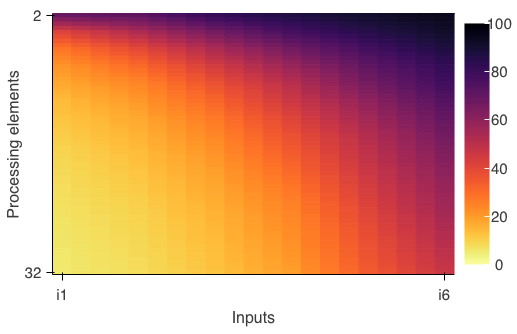
\includegraphics[width=\textwidth]{pascalanalyzer/figures/results/efficiency_raytrace.png}
%		\caption{\centering}
		\label{fig:efficiency_raytrace}
	\end{subfigure}
	\begin{subfigure}[b]{0.46\textwidth}
		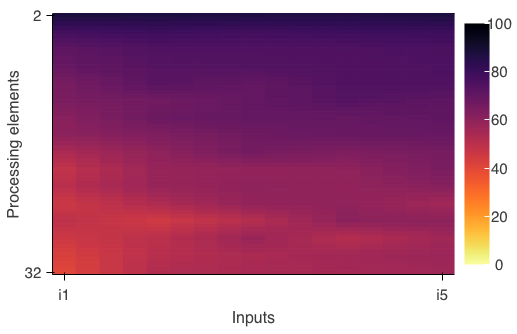
\includegraphics[width=\textwidth]{pascalanalyzer/figures/results/efficiency_openmc.png}
%		\caption{\centering}
		\label{fig:efficiency_openmc}
	\end{subfigure}
	
	\caption{Efficiency diagram varying the input size and the number of cores. The color bar indicates the efficiency value in percentage. (\textbf{a}) Raytrace efficiency diagram. (\textbf{b}) OpenMC efficiency diagram.}
	\label{fig:efficiency_all}
\end{figure}

The input values shown in Figures~\ref{fig:speedup}--\ref{fig:efficiency_all} indicate different data sets for processing. For example, the ``input 2'' represents a load that will require sequential processing with runtime twice as long as ``input 1''. Likewise, the ``input 3'' represents a load that will require sequential processing with runtime twice as long as ``input 2'', and so on.

Even if the analyzer does not display graphics natively, analysis aimed at observing scalability and energy consumption of applications depends on precise measurements, reinforcing the advantage of the analyzer proposed in this work.

% \begin{figure}[H]
% \centering
% 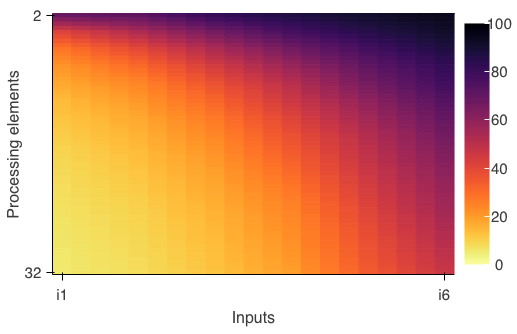
\includegraphics[width=\linewidth]{pascalanalyzer/figures/results/efficiency_raytrace.png}
% \caption{Efficiency for Raytrace}
% \label{fig:efficiency_raytrace}
% \end{figure}

% \begin{figure}[H]
% \centering
% 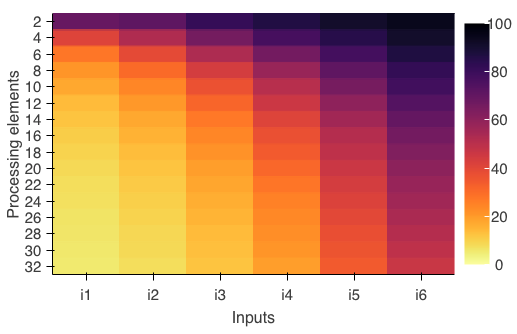
\includegraphics[width=\linewidth]{pascalanalyzer/figures/results/efficiency_raytrace_detailed.png}
% \caption{Efficiency for Raytrace}
% \label{fig:efficiency_raytrace_detailed}
% \end{figure}

% \begin{figure}[H]
% \centering
% 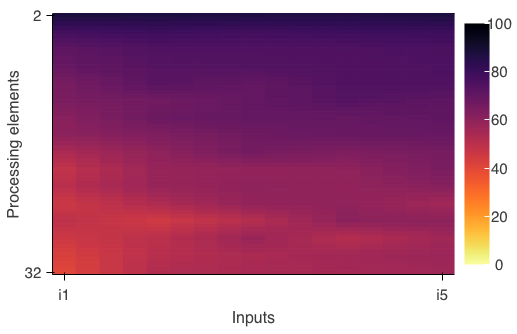
\includegraphics[width=\linewidth]{pascalanalyzer/figures/results/efficiency_openmc.png}
% \caption{Efficiency for OpenMC}
% \label{fig:efficiency_openmc}
% \end{figure}

% \begin{figure}[H]
% \centering
% 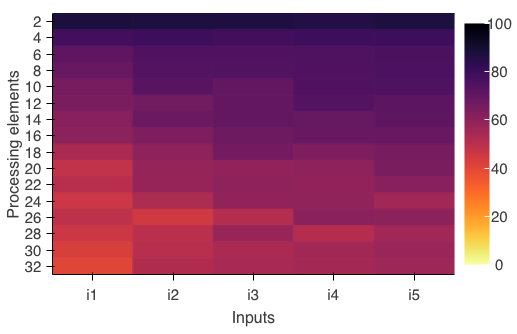
\includegraphics[width=\linewidth]{pascalanalyzer/figures/results/efficiency_openmc_detailed.png}
% \caption{Efficiency for OpenMC}
% \label{fig:efficiency_openmc_detailed}
% \end{figure}
\section{PMC Module validation} \label{sec:fingerprint_tool_validation}

In this subsection, we first show the comparison between our tool and others already established, as well as the clustering process.

%\subsection{Accuracy comparison} \label{subsec:ftv_accuracy_comparison}

% \begin{table*}[h]
% \centering
% \caption{Average}
% \begin{tabular}{|c|c|c|c|c|c|c|}
% \hline
% Counter                                 & Pined values & Linux API   & PAPI      & PAPI Python & Perf tool   & MyPerf      \\ \hline
% INSTRUCTIONS\_RETIRED                  & 226990030    & 227000691   & 227000620 & 225901249   & 227000572   & 227000650   \\ \hline
% BRANCH\_INSTRUCTIONS\_RETIRED          & 9240000      & 9250617     & 9250566   & 9239617     & 9250552     & 9250501     \\ \hline
% BR\_INST\_RETIRED:CONDITIONAL          & 8220000      & 8220000     & 8220000   & 8209717     & 8220000     & 8220000     \\ \hline
% MEM\_UOP\_RETIRED:ANY\_LOADS           &              & 2484182672  &           &             & 2484383940  & 2484155029  \\ \hline
% MEM\_UOP\_RETIRED:ANY\_STORES          &              & 189962002   &           &             & 189961539   & 189961321   \\ \hline
% UOPS\_RETIRED:ANY                      &              & 12291082129 &           &             & 12290811038 & 12290901997 \\ \hline
% PARTIAL\_RAT\_STALLS:MUL\_SINGLE\_UOP  &              & 600878      &           &             & 600151      & 600330      \\ \hline
% ARITH:FPU\_DIV                         &              & 5801446     &           &             & 5801000     & 5800977     \\ \hline
% FP\_COMP\_OPS\_EXE:X87                 &              & 48785528    &           &             & 48784834    & 48786021    \\ \hline
% INST\_RETIRED:X87                      &              & 17200008    &           &             & 17200008    & 17200007    \\ \hline
% FP\_COMP\_OPS\_EXE:SSE\_SCALAR\_DOUBLE &              & 5401694     &           &             & 5401842     & 5401679     \\ \hline
% \end{tabular}
% \label{tab:mean}
% \end{table*}

% \begin{table*}[h]
% \centering
% \caption{Standard deviation}
% \begin{tabular}{|c|c|c|c|c|c|}
% \hline
% Counter                                    & Linux API & PAPI & PAPI Python & Perf tool & MyPerf \\ \hline
% INSTRUCTIONS\_RETIRED                  & 396       & 133  & 337763      & 110       & 175    \\ \hline
% BRANCH\_INSTRUCTIONS\_RETIRED          & 297       & 208  & 8485        & 379       & 91     \\ \hline
% BR\_INST\_RETIRED:CONDITIONAL          & 0         & 0    & 3383        & 0         & 0      \\ \hline
% MEM\_UOP\_RETIRED:ANY\_LOADS           & 37399     &      &             & 39217     & 38953  \\ \hline
% MEM\_UOP\_RETIRED:ANY\_STORES          & 1513      &      &             & 1035      & 687    \\ \hline
% UOPS\_RETIRED:ANY                      & 345246    &      &             & 335832    & 333298 \\ \hline
% PARTIAL\_RAT\_STALLS:MUL\_SINGLE\_UOP  & 1222      &      &             & 252       & 521    \\ \hline
% ARITH:FPU\_DIV                         & 1760      &      &             & 1621      & 1544   \\ \hline
% FP\_COMP\_OPS\_EXE:X87                 & 1283      &      &             & 1920      & 3311   \\ \hline
% INST\_RETIRED:X87                      & 4         &      &             & 4         & 3      \\ \hline
% FP\_COMP\_OPS\_EXE:SSE\_SCALAR\_DOUBLE & 1547      &      &             & 3259      & 2097   \\ \hline
% \end{tabular}
% \label{tab:std}
% \end{table*}

\begin{table}[H]
	\centering
	\caption{Comparison}
	\resizebox{\textwidth}{!}{%
		\begin{tabular}{llllllllll}
			\hline
			\multicolumn{6}{l|}{\textbf{Average*$10^{-6}$}} & \multicolumn{4}{l}{\textbf{Standard deviation}}\\ \hline
			\textbf{Counters} & \begin{tabular}{l}\textbf{Pined} \\ \textbf{values}\end{tabular} & \begin{tabular}{l}\textbf{Linux} \\ \textbf{API}\end{tabular} & \textbf{PAPI} & \begin{tabular}{l}\textbf{PAPI} \\ \textbf{Python}\end{tabular} & \textbf{MyPerf}  & \begin{tabular}{|l}\textbf{Linux} \\ \textbf{API}\end{tabular} & \textbf{PAPI} & \begin{tabular}{l}\textbf{PAPI} \\ \textbf{Python}\end{tabular} & \textbf{MyPerf} \\ \hline
			INSTRUCTIONS\_RETIRED                  & 226.99       & 227       & 227  & 225.9       & 227     & 396       & 133  & 337763      & 175    \\
			BRANCH\_INSTRUCTIONS\_RETIRED          & 9.24         & 9.25      & 9.25 & 9.24        & 9.25    & 297       & 208  & 8485        & 91     \\
			BR\_INST\_RETIRED:CONDITIONAL          & 8.22         & 8.22      & 8.22 & 8.21        & 8.22    & 0         & 0    & 3383        & 0      \\
			MEM\_UOP\_RETIRED:ANY\_LOADS           &              & 2484.18   &      &             & 2484.16 & 37399     &      &             & 38953  \\
			MEM\_UOP\_RETIRED:ANY\_STORES          &              & 189.96    &      &             & 189.96  & 1513      &      &             & 687    \\
			UOPS\_RETIRED:ANY                      &              & 12291.08  &      &             & 12290.9 & 345246    &      &             & 333298 \\
			PARTIAL\_RAT\_STALLS:MUL\_SINGLE\_UOP  &              & 0.6       &      &             & 0.6     & 1222      &      &             & 521    \\
			ARITH:FPU\_DIV                         &              & 5.8       &      &             & 5.8     & 1760      &      &             & 1544   \\
			FP\_COMP\_OPS\_EXE:X87                 &              & 48.79     &      &             & 48.79   & 1283      &      &             & 3311   \\
			INST\_RETIRED:X87                      &              & 17.2      &      &             & 17.2    & 4         &      &             & 3      \\
			FP\_COMP\_OPS\_EXE:SSE\_SCALAR\_DOUBLE &              & 5.4       &      &             & 5.4     & 1547      &      &             & 2097   \\ \hline
		\end{tabular}
	}
	\label{tab:counters}
\end{table}

To validate the tool, we compared the results of the counters obtained with different APIs. 
We used the hand-crafted assembly benchmark from \cite{Weaver2013Non-determinismImplementations}, designed to test determinism and accuracy of PMUs.
We compared the values obtained from the Linux API, PAPI on C and PAPI on Python. 
The events used for this comparison were instructions retired, branch instructions, memory read, memory load, and arithmetic operations.
We ran the benchmark 30 times and calculated the mean and standard deviation as shown in table \ref{tab:counters}. Some events could not be measured using PAPI because the tool does not accept raw events and there are no equivalent events.

Since the benchmark was hand-crafted with assembly, we know exactly the value for some counter events. 
For this reason, the number of instructions, branch instructions, and conditional branch are pin. However, some other events are architecture-specific and there is no pined value. 
In the latter case, we can still compare to the Linux API, which should be closest to the reality.

The differences using the Linux low-level API, PAPI, and our tool are negligible (the average percentage distance is less than 0.01\% in all the cases). 
As expected, PAPI on Python had the largest difference (with an average distance of 0.25\%) mainly due to an unsynchronized start that resulted in the loss of some instructions at the beginning of the execution. 
This can be an important problem if the application contains a small number of instructions.

The standard deviation of the 30 executions shows that our tool has the smallest variation on a run-to-run on most events. On the contrary, PAPI on Python shows a big variation compared to the others.

\subsubsection{Case of study} \label{subsec:ftv_case_of_study}

To cluster applications first we need to have a way to compare two programs, for that we define a new variable that tries to compute a fingerprint to the program, this variable has to look similar when we execute the same program with different conditions and inputs. Thinking in the simplest model of a program as a Turing machine as everything can be done with a tap of memory and set of rules we empirically define the variable input size as described on the equation \ref{eq:input_size}. On real computers this is not too far from reality, most of the computations and input and output operations somehow pass through the memory, so analyzing the relationship of the total number of instructions and memory instructions can give us a good fingerprint.

\begin{equation}
	I_{sz} = \frac{I}{I_{m}} \\
	\label{eq:input_size}
\end{equation}

Where $I_{sz}$ we called input size, $I$ the number of instructions executed, $I_m$ number of memory instructions execute. We observe that this variable demonstrate to have the proprieties that we are looking for, produce similar results to the same program with different input size, and environment. This can be used to identify programs but also to see the similarities between different applications.

To compute the distance between two programs we use the Canberra metric \cite{Jurman2009CanberraLists}, described on the equation \ref{eq:canberra}.

\begin{equation}
	d(p,q)= \sum_{i=1}^{n}{\frac{|p_i-q_i|}{|p_i|+|q_i|}}
	\label{eq:canberra}
\end{equation}

Where $p$ and $q$ are n-dimensional vectors.

We compute the input size for all 30 applications of the Polybench with 3 different inputs. Running each program 15 times, with a sampling rate of 0.01 seconds collecting the total number of instruction, number of loads and write instructions, number of floating point operations, besides some software counters. After applying the post-processing to the data collected we compute the input size and perform a Hierarchical clustering using the linkage method of Ward \cite{Murtagh2011WardsAlgorithm}, that minimizes the total within-cluster variance. The results of the clustering can be seen on the figure \ref{fig:sping_force_is} and on the dendrogram on figure \ref{fig:dendograma_input_size}.

%The exact HPCs was:
%PERF_COUNT_HW_INSTRUCTIONS,
%MEM_UOPS_RETIRED:ALL_LOADS,
%MEM_UOPS_RETIRED:ALL_STORES,
%FP_ARITH_INST_RETIRED:SCALAR

\begin{figure*}[h]
	\centering
	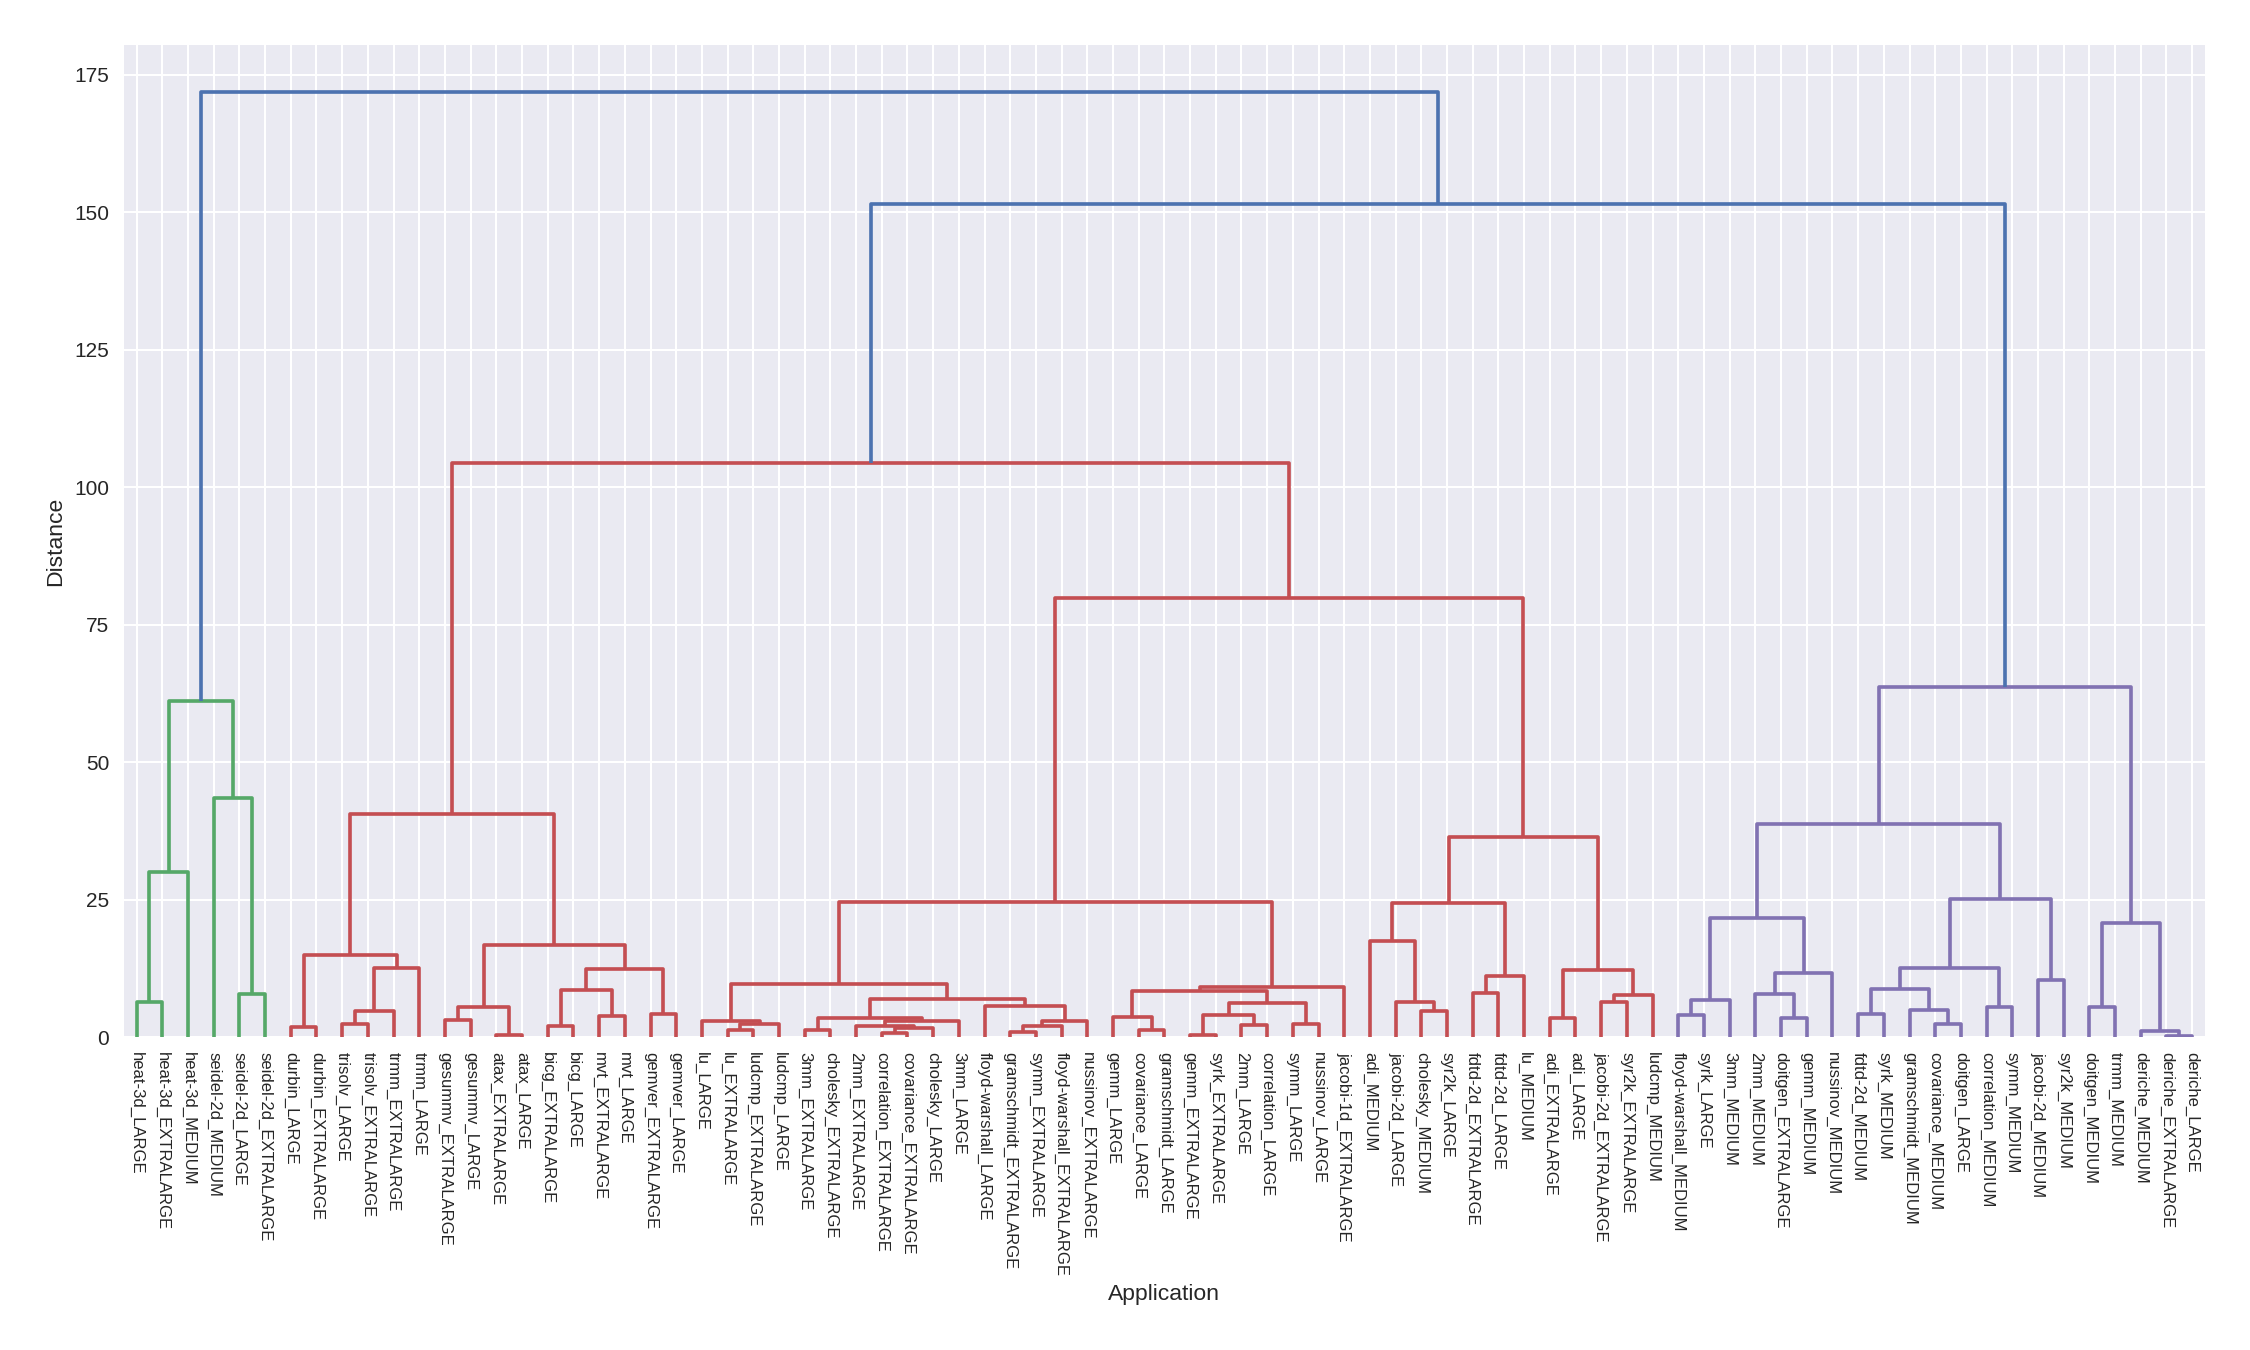
\includegraphics[width=\textwidth]{fingerprint/figures/dendograma_input_size.png}
	\caption{Dendrogram}
	\label{fig:dendograma_input_size}
\end{figure*}

From this dendrogram, we can have an idea of how close two applications are. We choose the number of clusters that maximize the number of hits of the same program with different input sizes on the same cluster, in this case, was 5 clusters.

It was observed that as input size grows the program behavior tends to a specific curve, but for small input sizes some have variation, so in some cases, the same program has been classified in more than one cluster. This can also happen if specific parts of the program are triggered with specific inputs, in which case it will also belong to more than one cluster.

In order to have an overall classification of each program, we can pick up the frequency in which each appeared in the clusters and classified it in the cluster in which it appeared more often. In this case, the clusters are:

\begin{itemize}
	\item Cluster 1: 2mm, 3mm, cholesky, correlation, covariance, floyd-warshall, gemm, gramschmidt, lu, ludcmp, nussinov, symm
	
	\item Cluster 2: deriche, doitgen, syrk
	
	\item Cluster 3: adi, fdtd-2d, jacobi-2d, syr2k
	
	\item Cluster 4: atax, bicg, durbin, gemver, gesummv, mvt, trisolv, trmm
	
	\item Cluster 5: heat-3d, seidel-2d
\end{itemize}

On the figure, \ref{fig:sping_force_is} we display the clusters using the spring force algorithm where each program with a specific input is a node and the edge weight is the Canberra distance. To a better visualization, the name of the inputs was replaced by numbers, the EXTRALARGE is 3, LARGE 2 and MEDIUM 1. 

\begin{figure}[H]
	\centering
	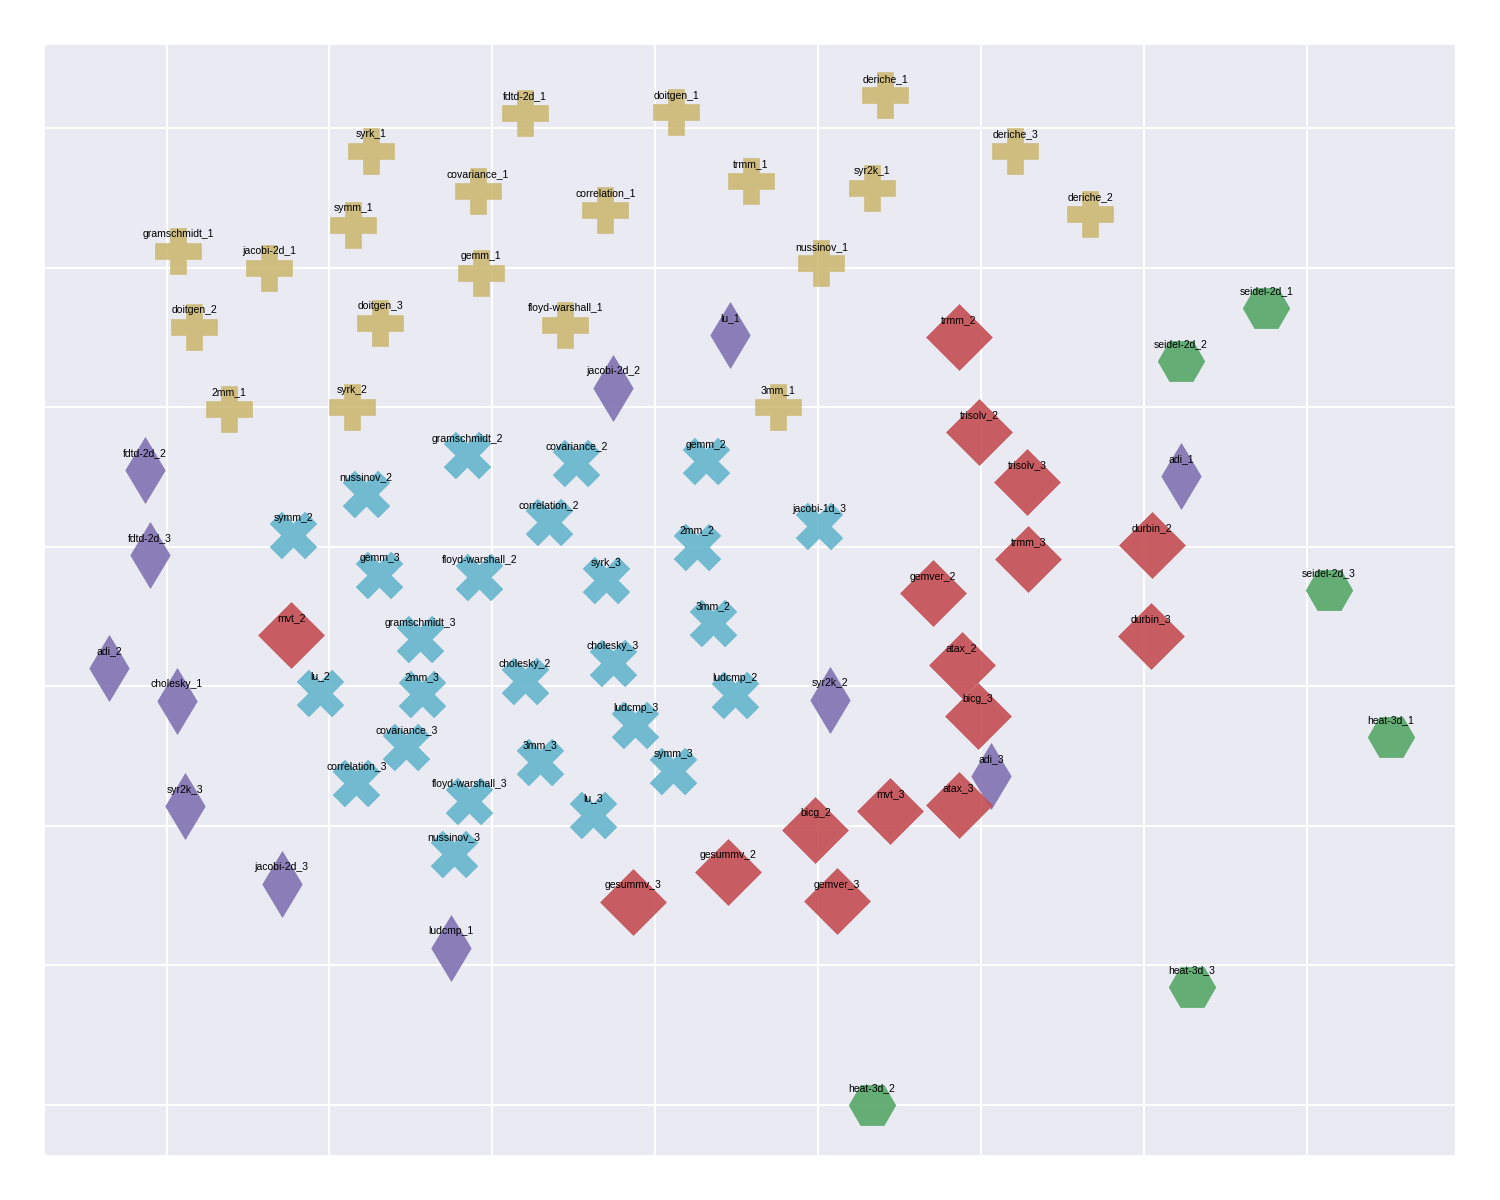
\includegraphics[width=\textwidth]{fingerprint/figures/graph_input_size.png}
	\caption{Spring force of Canberra distance}
	\label{fig:sping_force_is}
\end{figure}

The figure above shows a different way to observe in a reduced space the distance between clusters and applications and how they are organized. From this graph, we see that clustering it's well partitioned and we can clearly separate each cluster. It is also interesting to note that the applications of the cluster formed by the circle symbol are more separated, which may indicate that they were classified in this way because they did not fit into any other cluster.

% \begin{figure*}[t]
%     \begin{subfigure}{\textwidth}
%         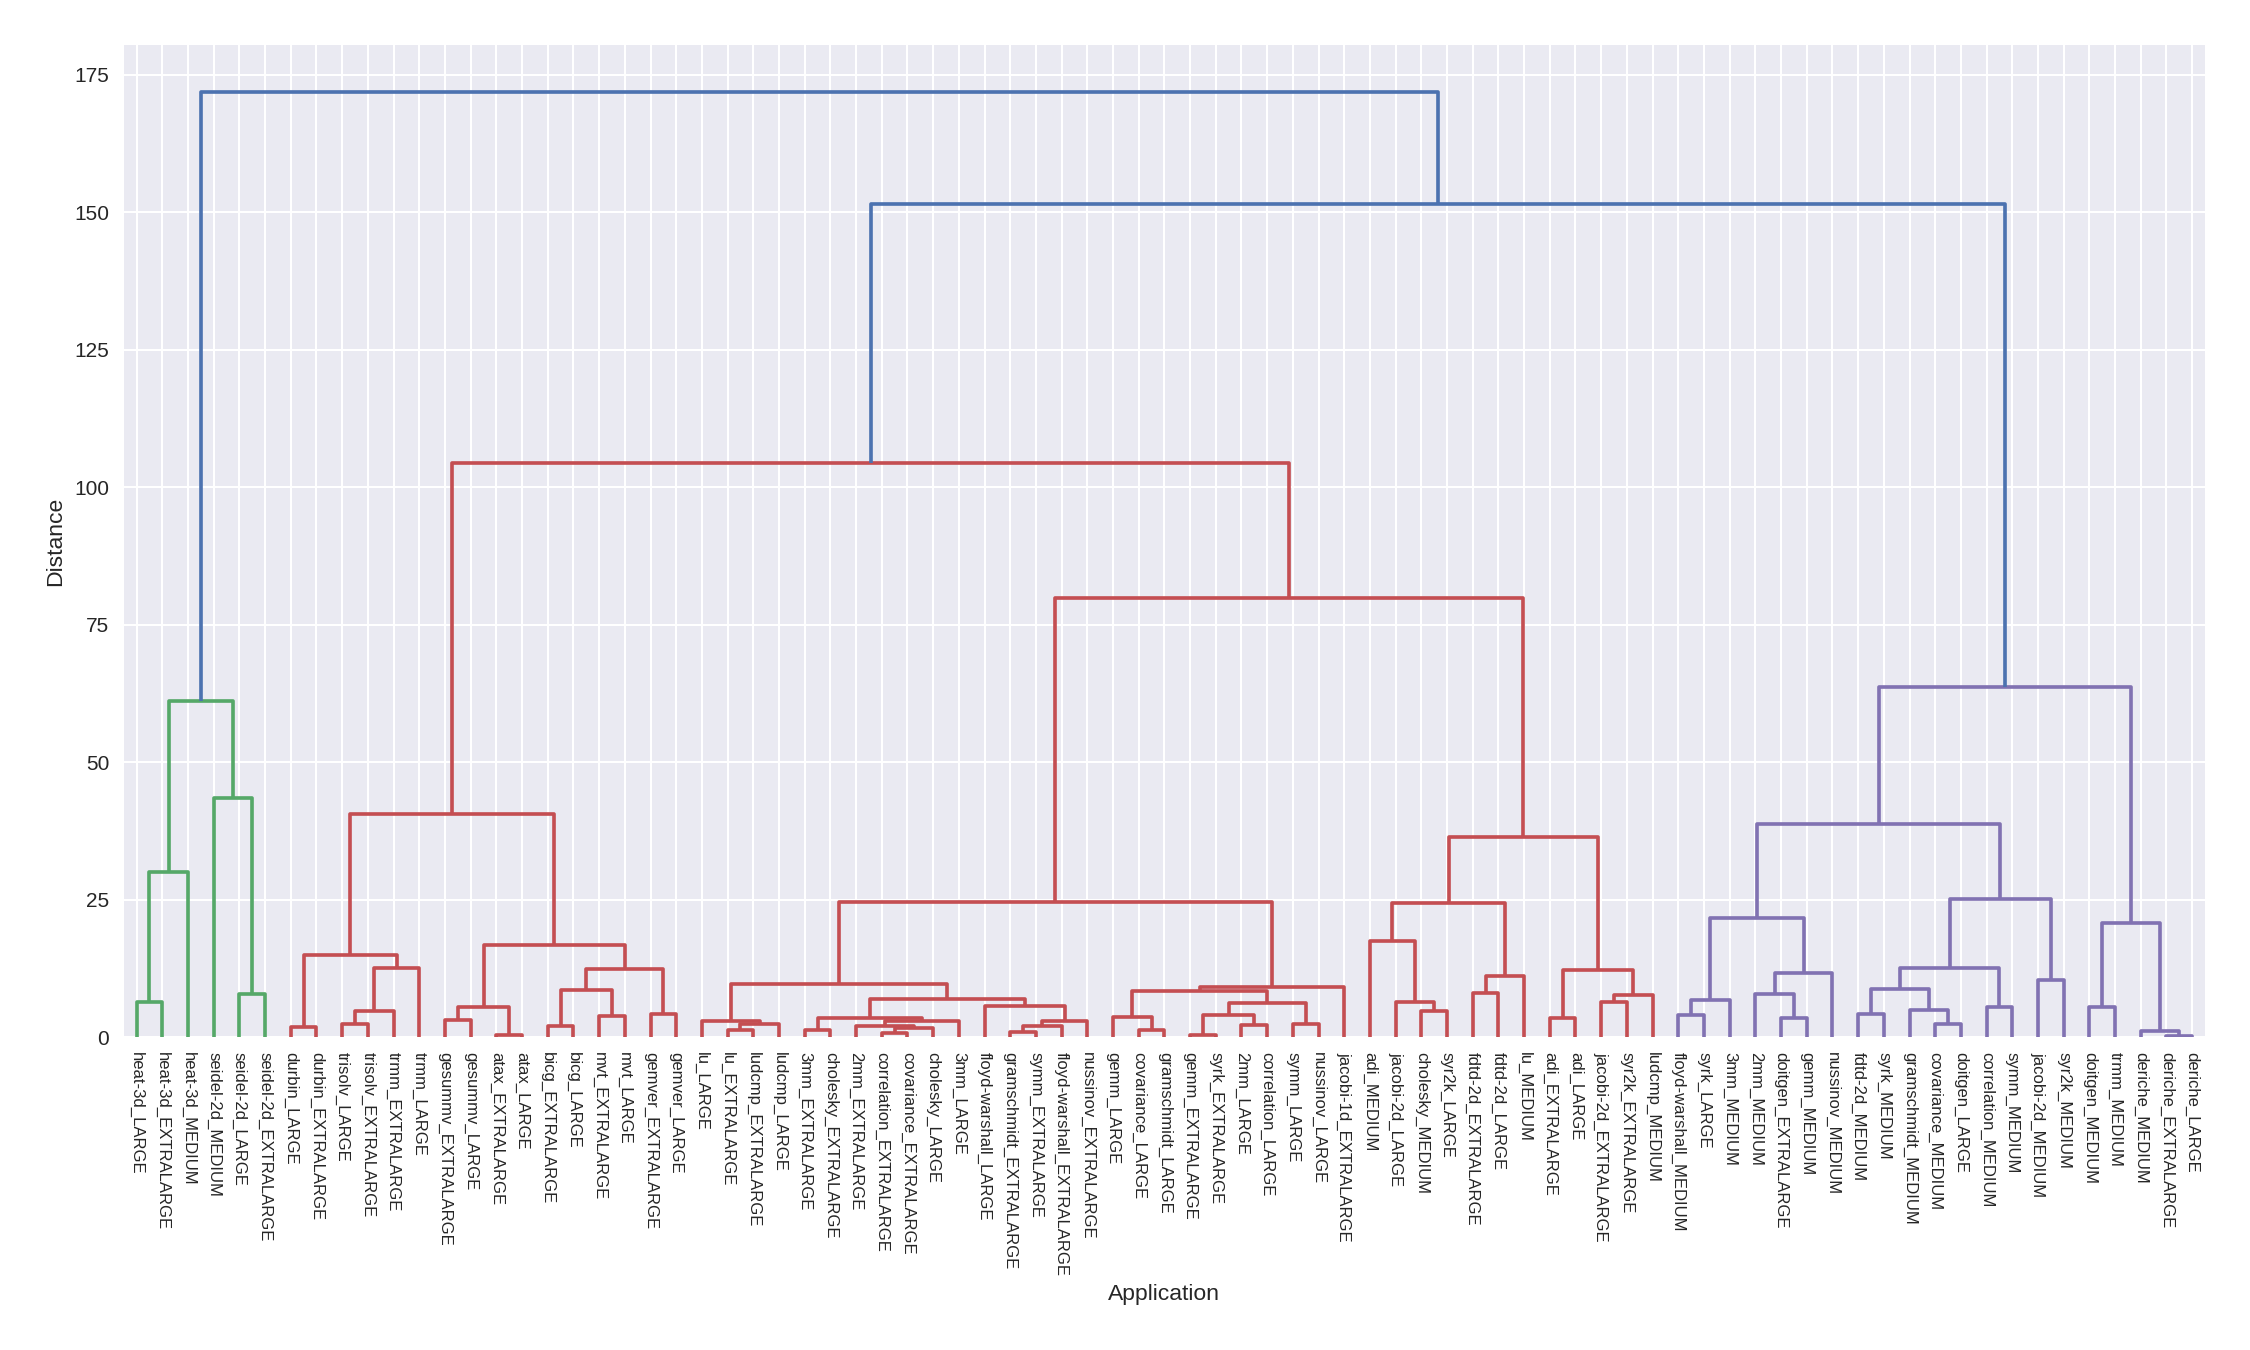
\includegraphics[width=\textwidth]{fingerprint/figures/dendograma_input_size.png}
%     \end{subfigure}
%     \\
%     \begin{subfigure}{\textwidth}
%         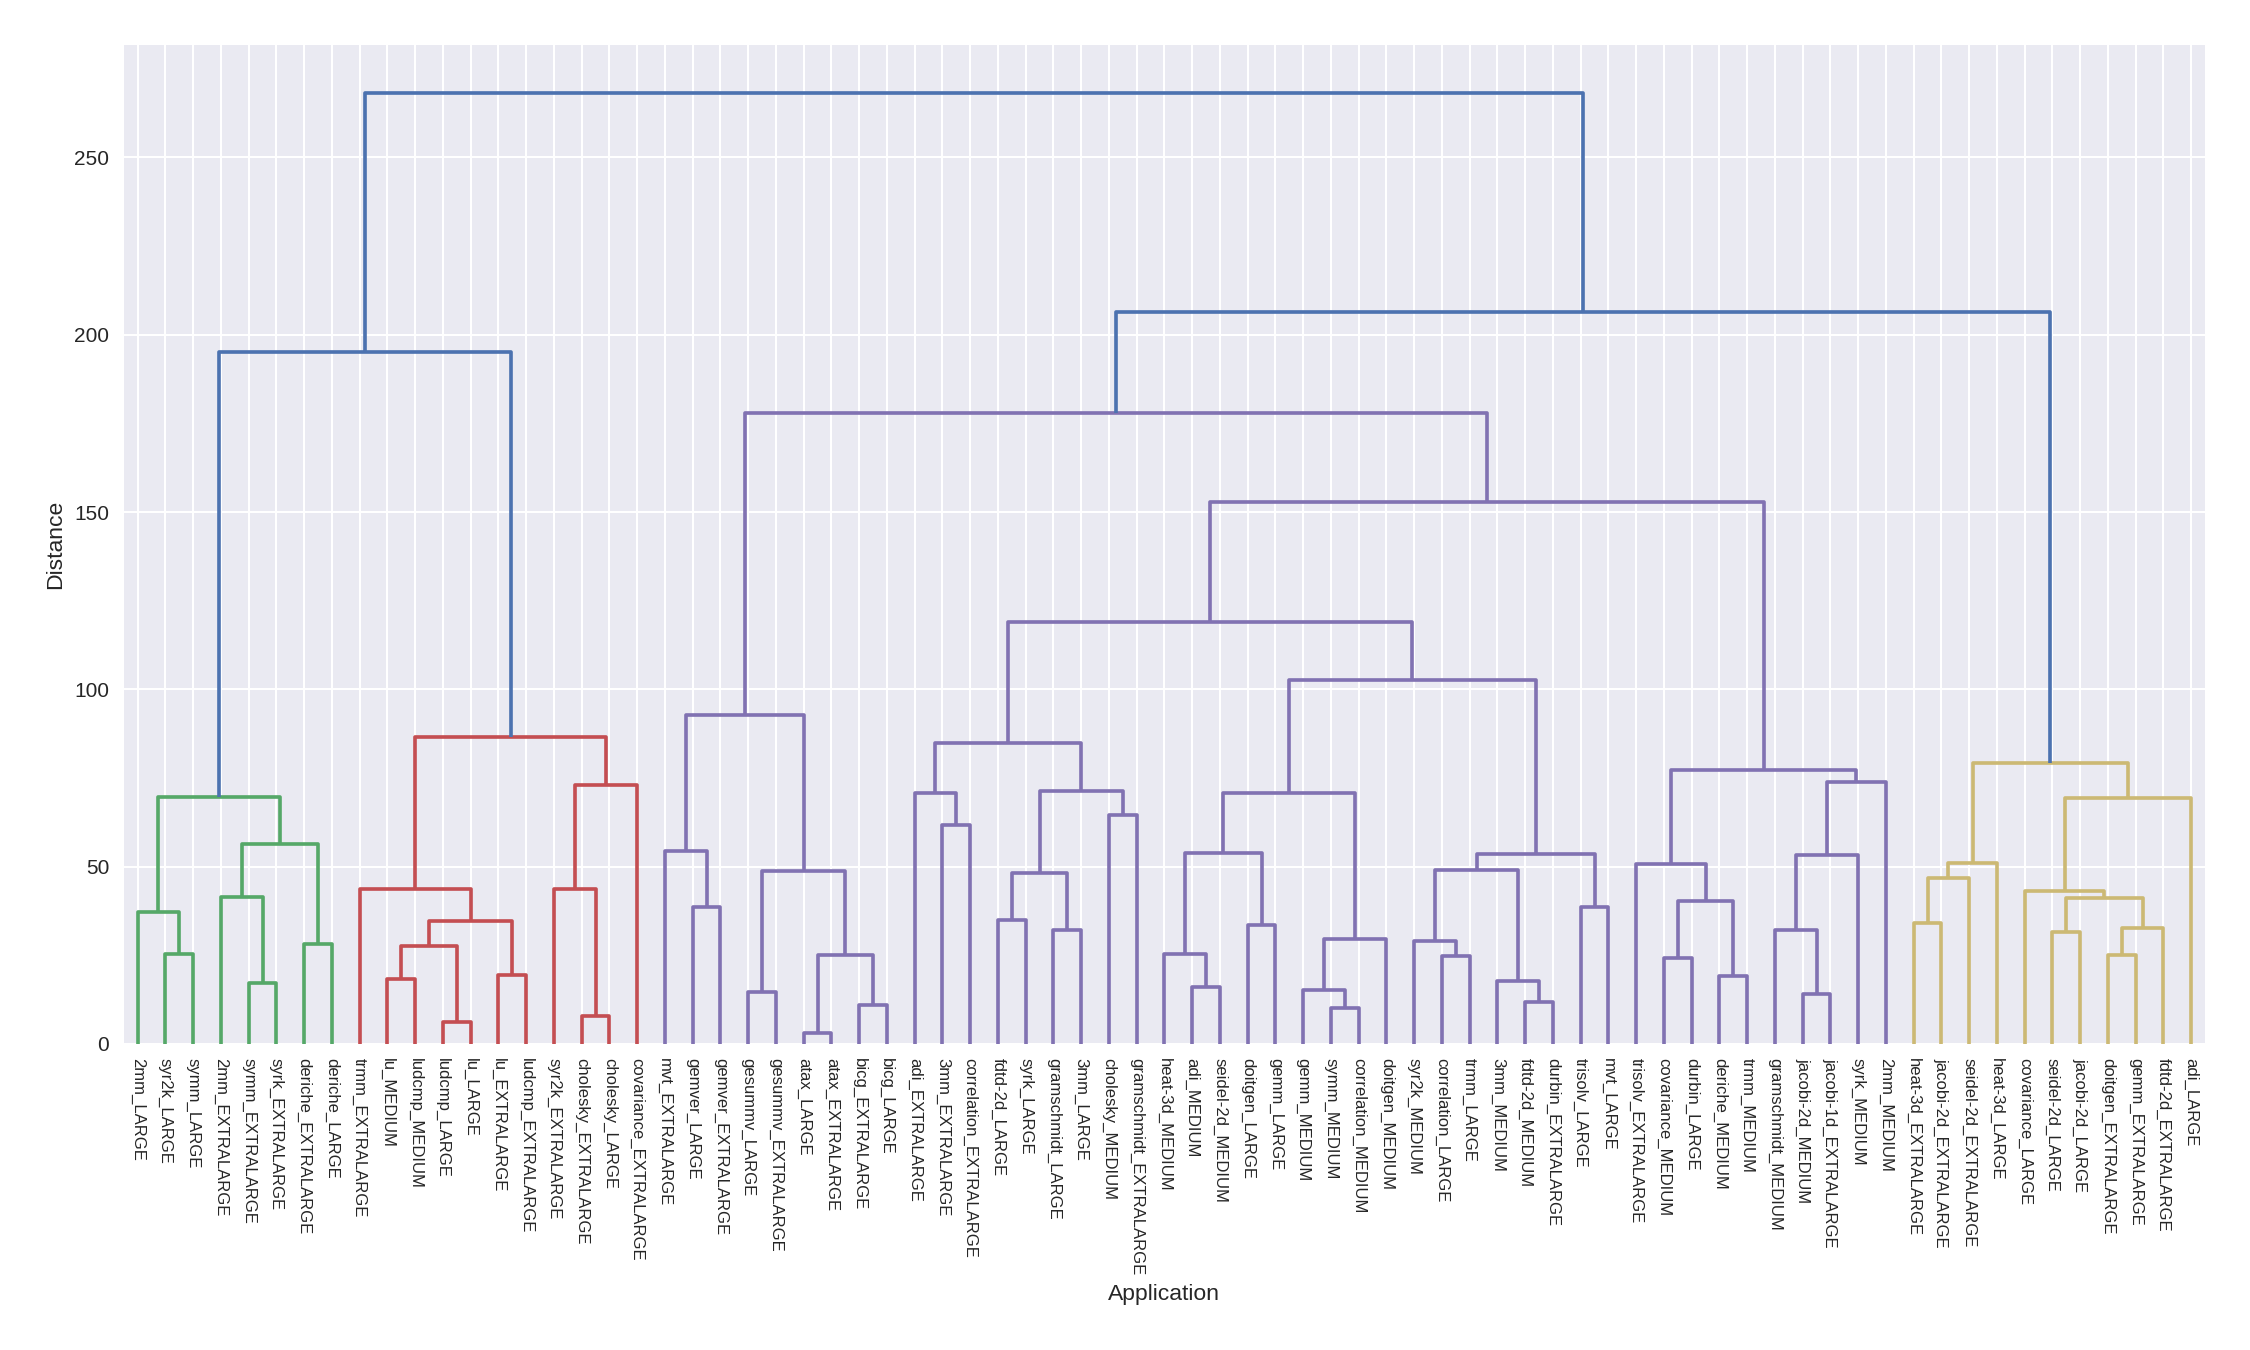
\includegraphics[width=\textwidth]{fingerprint/figures/dendograma_floating.png}
%     \end{subfigure}
%     %and so on
% \end{figure*}

To have an idea of how the behavior of the variable input size for each clusters is, it was plotted for the applications of clusters 1 and 2 shown on the figures \ref{fig:c1_input_size_0}, \ref{fig:c1_input_size_1}.

\begin{figure}[H]
	\centering
	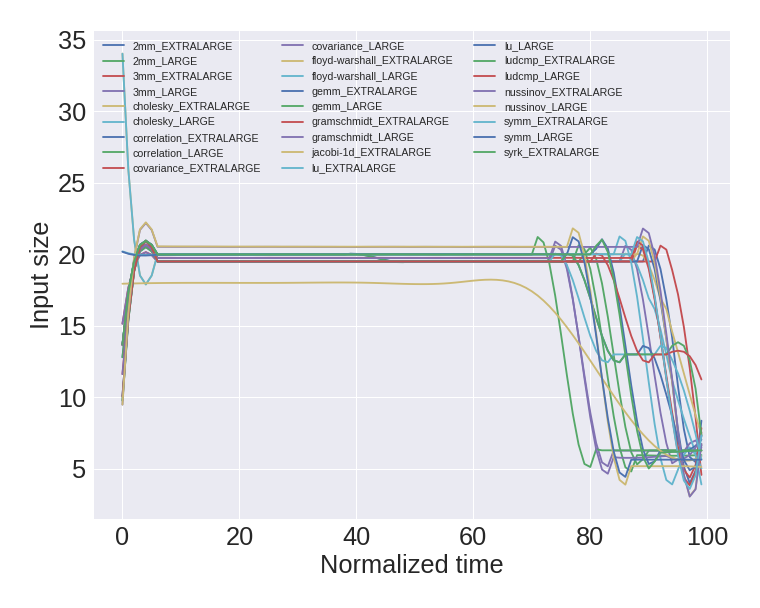
\includegraphics[width=\textwidth]{fingerprint/figures/cluster_input_0.png}
	\caption{Input size - Cluster 1}
	\label{fig:c1_input_size_0}
\end{figure}

From these figures, we can have an idea of what behavior was classified as the same class. On cluster 1 on the figure \ref{fig:c1_input_size_0} all applications showed the same behavior with approximately the same amplitude.

\begin{figure}[H]
	\centering
	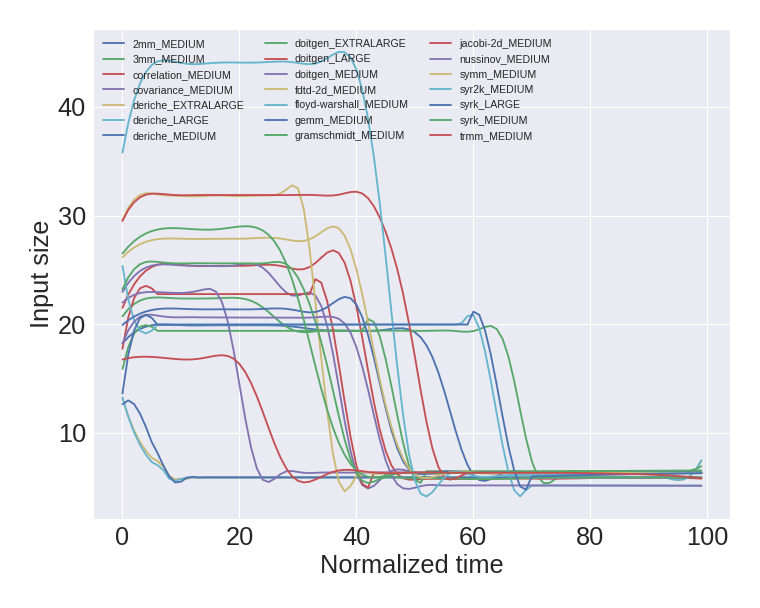
\includegraphics[width=\textwidth]{fingerprint/figures/cluster_input_1.png}
	\caption{Input size - Cluster 2}
	\label{fig:c1_input_size_1}
\end{figure}

On figure \ref{fig:c1_input_size_1} we observe that curves that have similar shape regardless of scale on vertical and horizontal axis have also been classified as the same clusters. This is the wanted comportment for the classification because we are only interested in the overall shape of the curve.


% \begin{figure}[H]
%     \centering
%     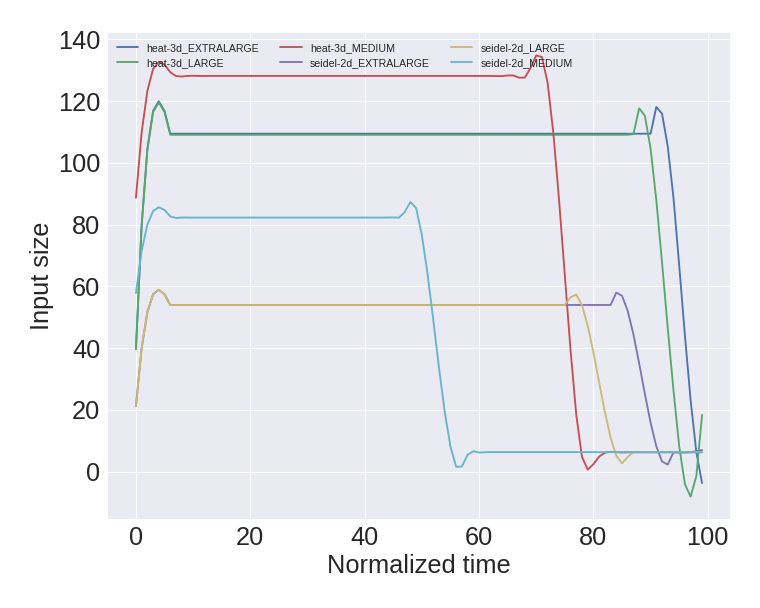
\includegraphics[width=\textwidth]{fingerprint/figures/cluster_input_4.png}
%     \caption{Input size - Cluster 3}
%     \label{fig:c1_input_size_2}
% \end{figure}

% To conclude this study we also clustering applications by its floating point behavior. For that we only use the counter correspondent to floating point operations. The figure \ref{fig:dendogram_fp} shows the dendrogram and the \ref{fig:sping_force_fp} the spring force graph plot.

% \begin{figure*}[h]
%     \includegraphics[width=\textwidth]{fingerprint/figuresdendograma_floating.png}
%     \caption{Dendrogram}
%     \label{fig:dendogram_fp}
% \end{figure*}

% \begin{figure}[H]
%     \centering
%     \includegraphics[width=\textwidth]{fingerprint/figures/graph_floating2.png}
%     \caption{Spring force of Canberra distance}
%     \label{fig:sping_force_fp}
% \end{figure}

% The figures \ref{fig:cluster_fp1},\ref{fig:cluster_fp2},\ref{fig:cluster_fp3} show the behavior on the same cluster for the float point operations. For this classification the number of clusters was 8.

% \begin{figure}[H]
%     \centering
%     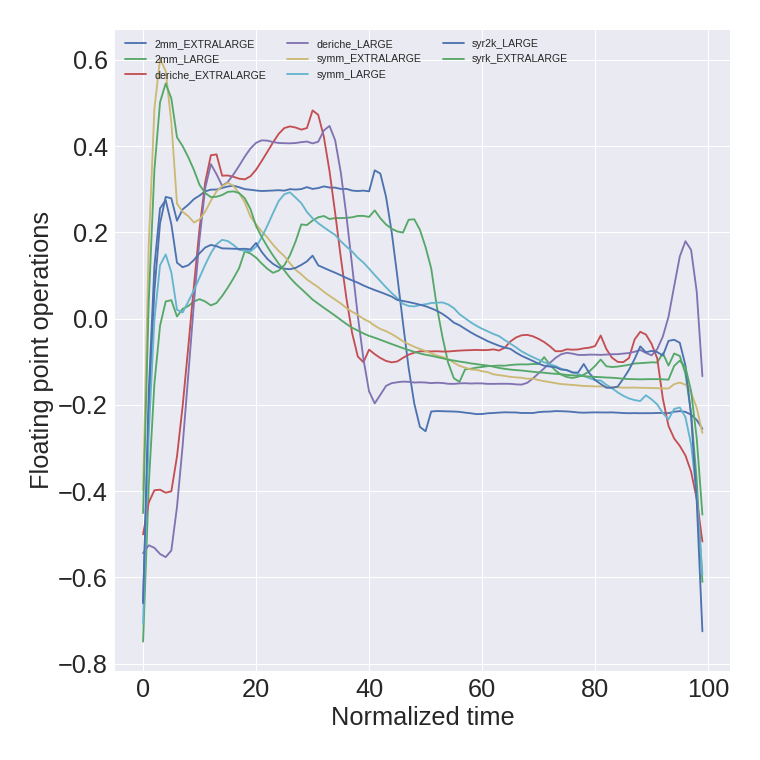
\includegraphics[width=\textwidth]{fingerprint/figures/cluster_fp_0.png}
%     \caption{Floating point - Cluster 1}
%     \label{fig:cluster_fp1}
% \end{figure}

% \begin{figure}[H]
%     \centering
%     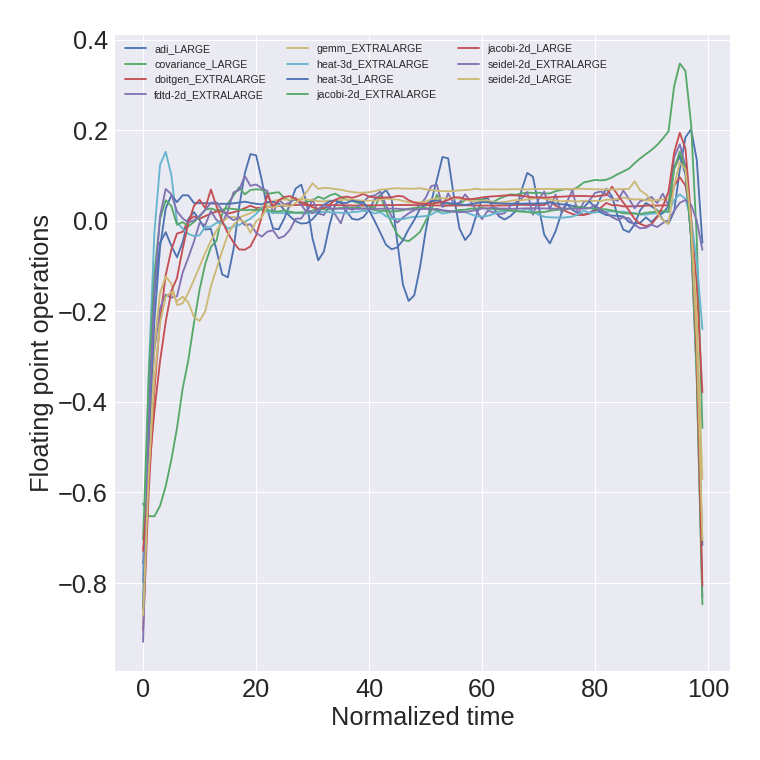
\includegraphics[width=\textwidth]{fingerprint/figures/cluster_fp_4.png}
%     \caption{Floating point - Cluster 2}
%     \label{fig:cluster_fp2}
% \end{figure}

% \begin{figure}[H]
%     \centering
%     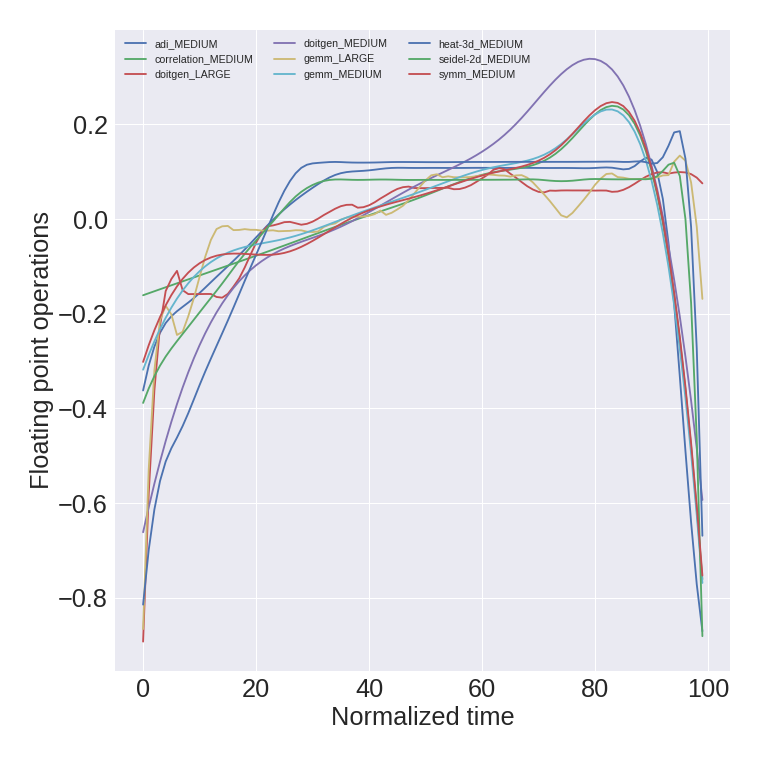
\includegraphics[width=\textwidth]{fingerprint/figures/cluster_fp_5.png}
%     \caption{Floating point - Cluster 3}
%     \label{fig:cluster_fp3}
% \end{figure}

% Here we can also observed again that applications with the same shape were classified as the same clusters.

